\begin{savequote}[45mm]
\ascii{Any fool can write code that a computer can understand. Good programmers write code that humans can understand.}
\qauthor{\ascii{- Martin Flower}}
\end{savequote}

\chapter{系统架构} 
\label{ch:architecture}

\begin{content}

本章将阐述\tf{}的系统架构,并一个简单的例子,讲述图结构的变换过程,加深理解\tf{}运行时的工作机理。

\end{content}

\section{系统架构}

\begin{content}

\tf{}的系统结构以\ascii{C API}为界,将整个系统分为「前端」和「后端」两个子系统:

\begin{enum}
  \eitem{前端系统:提供编程模型,负责构造计算图;}
  \eitem{后端系统:提供运行时环境,负责执行计算图。} 
\end{enum}

\begin{figure}[!htbp]
\centering
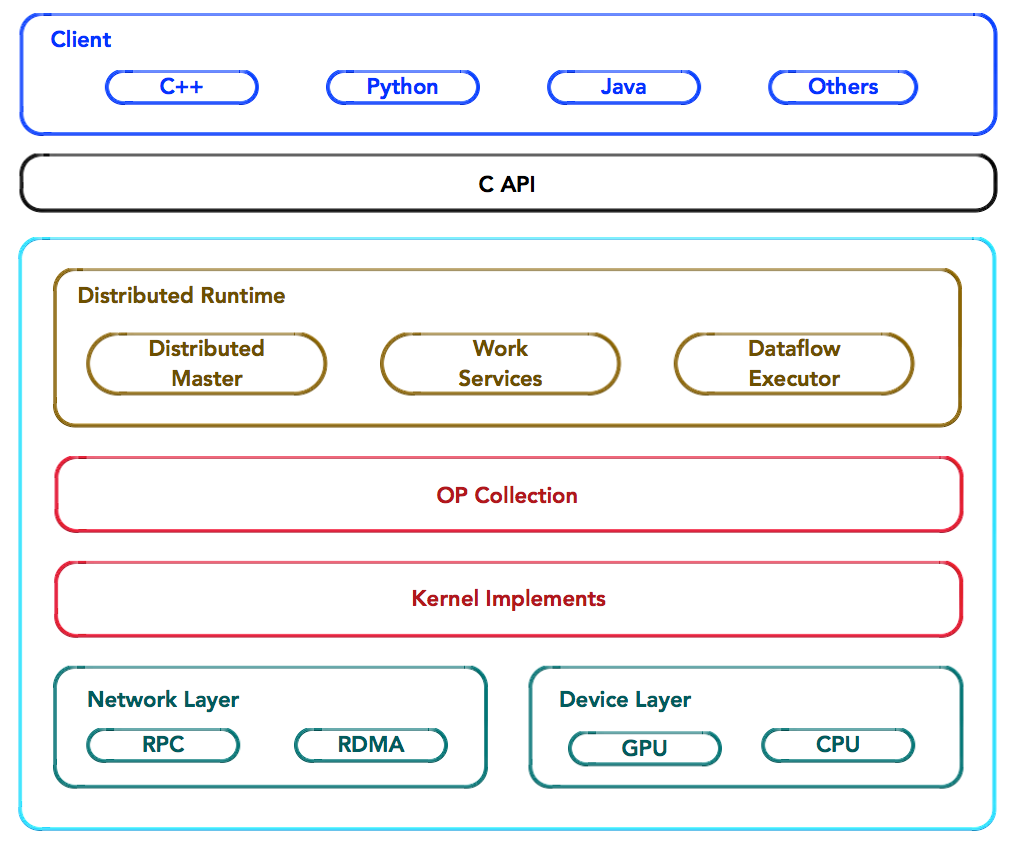
\includegraphics[width=0.9\textwidth]{figures/tf-architecture.png}
\caption{TensorFlow系统架构}
 \label{fig:tf-architecture}
\end{figure}

如\refig{tf-architecture}所示,重点关注系统中如下\ascii{4}个基本组件,它们是系统分布式运行时的核心。

\subsection{Client}

\ascii{Client}是前端系统的主要组成部分,它是一个支持多语言的编程环境。\ascii{Client}基于\ascii{TensorFlow}的编程接口,构造计算图。目前,\ascii{TensorFlow}支持\ascii{Python}和\ascii{C++}的编程接口较为完善,尤其对\ascii{Python}支持最佳;并且,对其他编程语言的编程接口的支持日益完善。

此时,\ascii{TensorFlow}并未执行任何的图计算,直至与后台计算引擎建立\ascii{Session},并以\ascii{Session}为桥梁,建立\ascii{Client}与\ascii{Master}之间的通道,将\ascii{Protobuf}格式的\ascii{GraphDef}发送至\ascii{Master},启动计算图的执行过程。

\subsection{Master}

在分布式的运行时环境中,\ascii{Client}根据\code{Session.run}传递整个计算图给后端的\ascii{Master};此时,计算图是完整的,常称为\ascii{Full Graph}。

随后,\ascii{Master}根据\ascii{Client}通过\code{Session.run}传递\code{fetches}参数列表,反向遍历\ascii{Full Graph},并按照依赖关系,对其实施剪枝,最终计算得到所依赖的「最小子图」,常称为\ascii{Client Graph}。

随后,\ascii{Master}负责将\ascii{Client Graph}按照任务的名称分裂\ascii{(split-by-task)}为多个「子图片段」,常称为\ascii{(Graph Partition)};其中,每个\ascii{Worker}对应一个\ascii{Graph Partition}。

随后,\ascii{Master}将\ascii{Graph Partition}分别注册到相应的\ascii{Worker}上,以便在不同的\ascii{Worker}上并发执行这些「子图片段」。

最后,\ascii{Master}将通知所有\ascii{Work}启动相应的\ascii{Graph Partition}的执行;其中,\ascii{Work}之间可能存在数据交互,\ascii{Master}不参与两者之间的数据交换,它们自行通信,独立交换数据即可,直至计算完成。

\subsection{Worker}

对于每以个任务,\tf{}都将启动一个\ascii{Worker}实例。\ascii{Worker}主要负责如下\ascii{3}个方面的职责:

\begin{enum}
  \eitem{处理来自\ascii{Master}的请求;}
  \eitem{调度\ascii{OP}的\ascii{Kernel}实现,执行本地子图;} 
  \eitem{协同任务之间的数据通信。}
\end{enum}

首先,\ascii{Worker}收到\ascii{Master}发送过来的图执行命令,此时的计算图相对于\ascii{Worker}是完整的,也称为\ascii{Full Graph},它对应于\ascii{Master}的一个\ascii{Graph Partition}。随后,\ascii{Worker}也会执行图剪枝,得到最小依赖的\ascii{Client Graph}。

随后,\ascii{Worker}根据当前可用的硬件环境,包括\ascii{(GPU/CPU)}资源,按照\ascii{OP}设备的约束规范,再将\ascii{Cliet Graph}分裂\ascii{(split-by-device)}为多个\ascii{Graph Partition};其中,每个计算设备对应一个\ascii{Graph Partition};随后,\ascii{Worker}启动所有当前设备的\ascii{Graph Partition}的执行。

最后,对于每一个计算设备,\ascii{Worker}将按照计算图中节点之间的依赖关系执行拓扑排序算法,并依次调用\ascii{OP}的\ascii{Kernel}实现,完成\ascii{OP}的运算(一种典型的多态实现技术)。其中,\ascii{Worker}还要负责将\ascii{OP}运算的结果发送到其他的\ascii{Work};或者接受来自其他\ascii{Worker}发送给它运算的结果,以便实现\ascii{Worker}之间的数据交互。

\subsection{Kernel}

\ascii{Kernel}是\ascii{OP}在某种硬件设备的特定实现,它负责执行\ascii{OP}的具体运算。目前,\ascii{TensorFlow}系统中包含\ascii{200}多个标准的\ascii{OP},包括数值计算,多维数组操作,控制流,状态管理等。

每一个\ascii{OP}根据设备类型都会存在一个优化了的\ascii{Kernel}实现。在运行时,运行时根据\ascii{OP}的设备约束贵方,及其本地设备的类型,为\ascii{OP}选择特定的\ascii{Kernel}实现,完成该\ascii{OP}的计算。

其中,大多数\ascii{Kernel}基于\ascii{Eigen::Tensor}实现。其中,\ascii{Eigen::Tensor}是一个使用\ascii{C++}模板技术,为多核\ascii{CPU/GPU}生成高效的并发代码。但是,\ascii{TensorFlow}也可以灵活地直接使用\ascii{cuDNN}实现更高效的\ascii{Kernel}。

此外,\ascii{TensorFlow}实现了矢量化技术,在高吞吐量、以数据为中心的应用需求中,及其移动设备中,实现更高效的推理。如果对于复合\ascii{OP}的子计算过程很难表示,或执行效率低下,\ascii{TensorFlow}甚至支持更高效的\ascii{Kernel}注册,其扩展性表现相当优越。

\end{content}

\section{图控制}

\begin{content}

随后,通过一个最简单的例子,进一步抽丝剥茧,逐渐挖掘出\tf{}计算图的控制与运行机制。


\subsection{组建集群}

如\refig{tf-1ps-1worker}所示。假如存在一个简单的分布式环境:\ascii{1 PS + 1 Worker},并将其划分为两个任务:

\begin{enum}
  \eitem{\ascii{ps0}: 使用\code{/job:ps/task:0}标记,负责模型参数的存储和更新;}
  \eitem{\ascii{worker0}: \code{/job:worker/task:0}标记,负责模型的训练。} 
\end{enum}

\begin{figure}[!htbp]
\centering
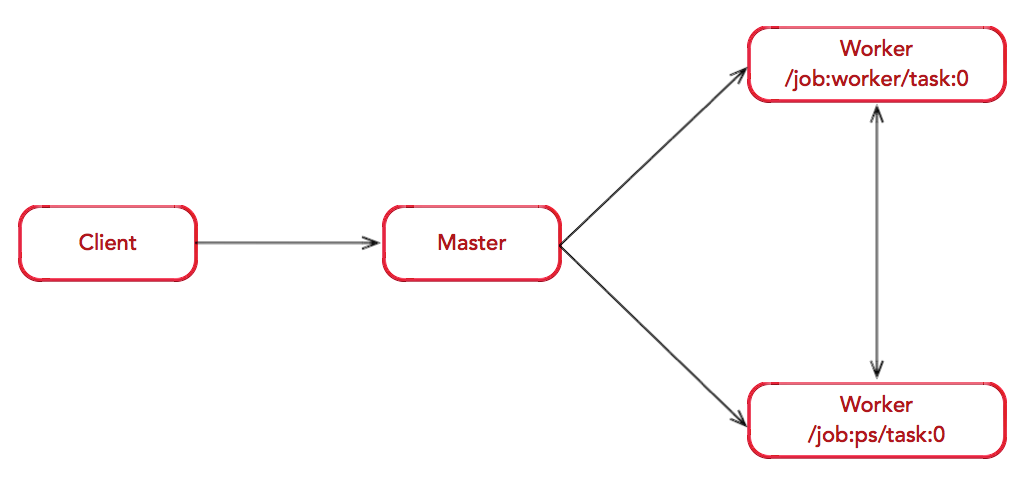
\includegraphics[width=0.9\textwidth]{figures/tf-1ps-1worker.png}
\caption{TensorFlow集群:\ascii{1 PS + 1 Worker}}
 \label{fig:tf-1ps-1worker}
\end{figure}

\subsection{图构造}

如\refig{tf-graph-construction}所示。\ascii{Client}构建了一个简单计算图;首先,将$w$与$x$进行矩阵相乘,再与截距$b$按位相加,最后更新至$s$。

\begin{figure}[!htbp]
\centering
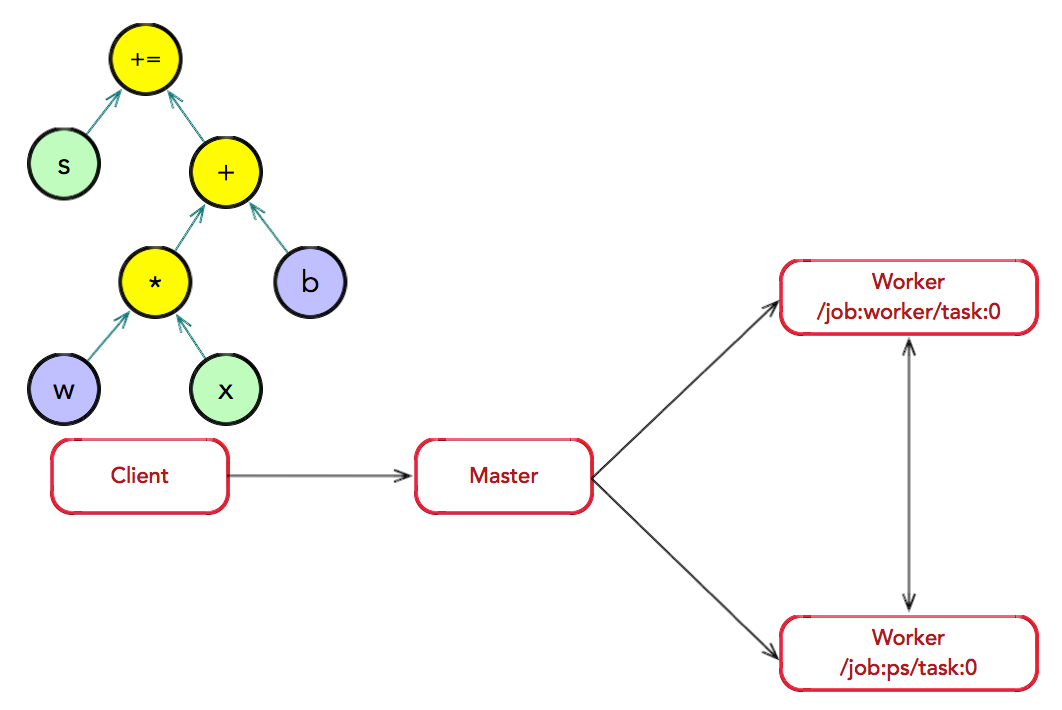
\includegraphics[width=0.9\textwidth]{figures/tf-graph-construction.png}
\caption{图构造}}
 \label{fig:tf-graph-construction}
\end{figure}

\subsection{图执行}

如\refig{tf-graph-execution}所示。首先,\ascii{Client}创建一个\code{Session}实例,建立与\ascii{Master}之间的通道;接着,\ascii{Client}通过调用\code{Sess.run}将计算图传递给\ascii{Master}。

随后,\ascii{Master}便开始启动一次\ascii{Step}的图计算过程。在执行之前,\ascii{Master}会实施一系列优化技术,例如「公共表达式消除」,「常量折叠」等。最后,\ascii{Master}负责任务之间的协同,执行优化后的计算子图。

\begin{figure}[!htbp]
\centering
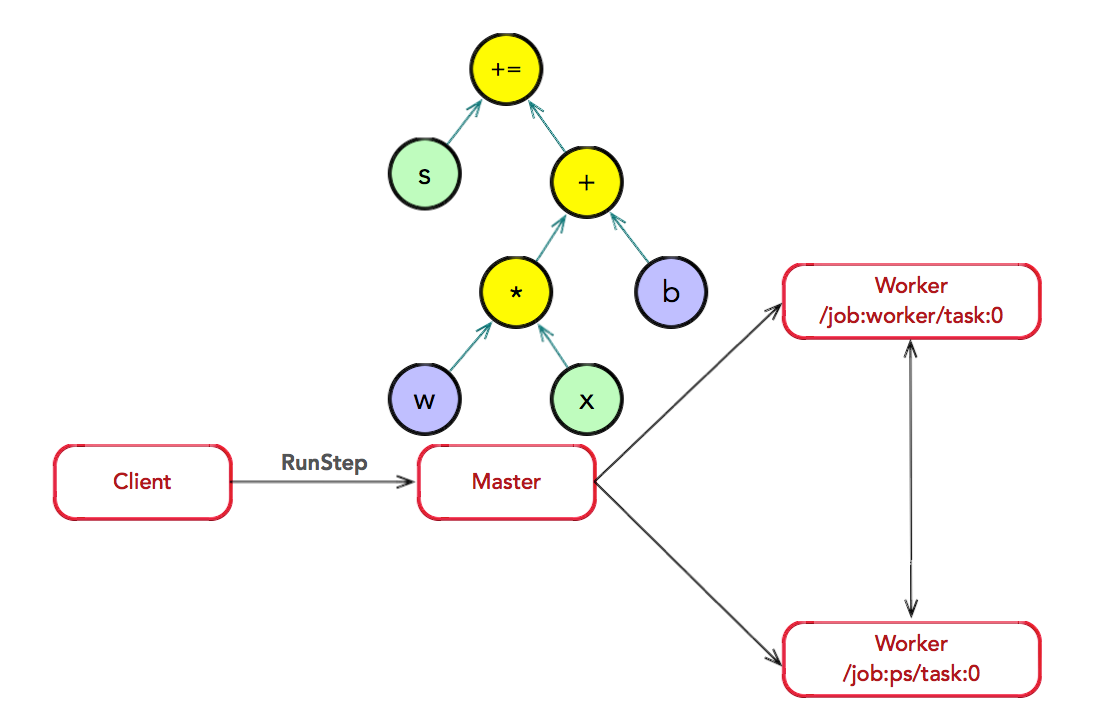
\includegraphics[width=0.9\textwidth]{figures/tf-graph-execution.png}
\caption{图执行}}
 \label{fig:tf-graph-execution}
\end{figure}

\subsubsection{图分裂}

如\refig{tf-graph-split-by-task}所示。存在一种合理的图划分算法。\ascii{Master}将模型参数相关的\ascii{OP}划分为一组,并放置在\ascii{ps0}任务上;其他\ascii{OP}划分为另外一组,放置在\ascii{worker0}任务上执行。

\begin{figure}[!htbp]
\centering
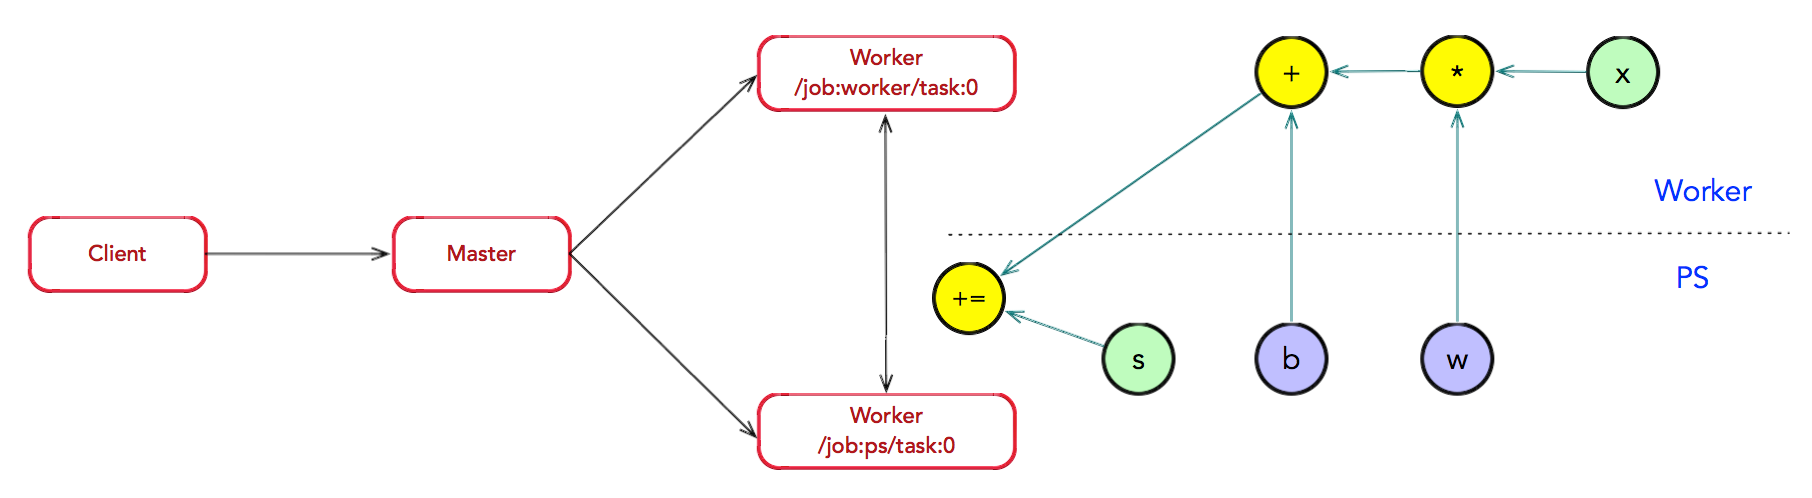
\includegraphics[width=0.9\textwidth]{figures/tf-graph-split-by-task.png}
\caption{图分裂:按任务划分}}
 \label{fig:tf-graph-split-by-task}
\end{figure}

\subsubsection{子图注册}

如\refig{tf-register-graph}所示。在图分离过程中,如果计算图的边跨越任务节点,\ascii{Master}将该边进行分裂,在两个任务之间插入\ascii{Send}和\ascii{Recv}节点,实现数据的传递。

其中,\ascii{Send}和\ascii{Recv}节点也是\ascii{OP},这是两个特殊的\ascii{OP},由内部运行时管理和控制,对用户不可见;并且,它们仅用于数据的通信,并没有任何数据计算的逻辑。

最后,\ascii{Master}通过调用\code{RegisterGraph}接口,将\ascii{Graph Partition}注册给相应的任务中,并由相应的\ascii{Worker}负责执行。

\begin{figure}[!htbp]
\centering
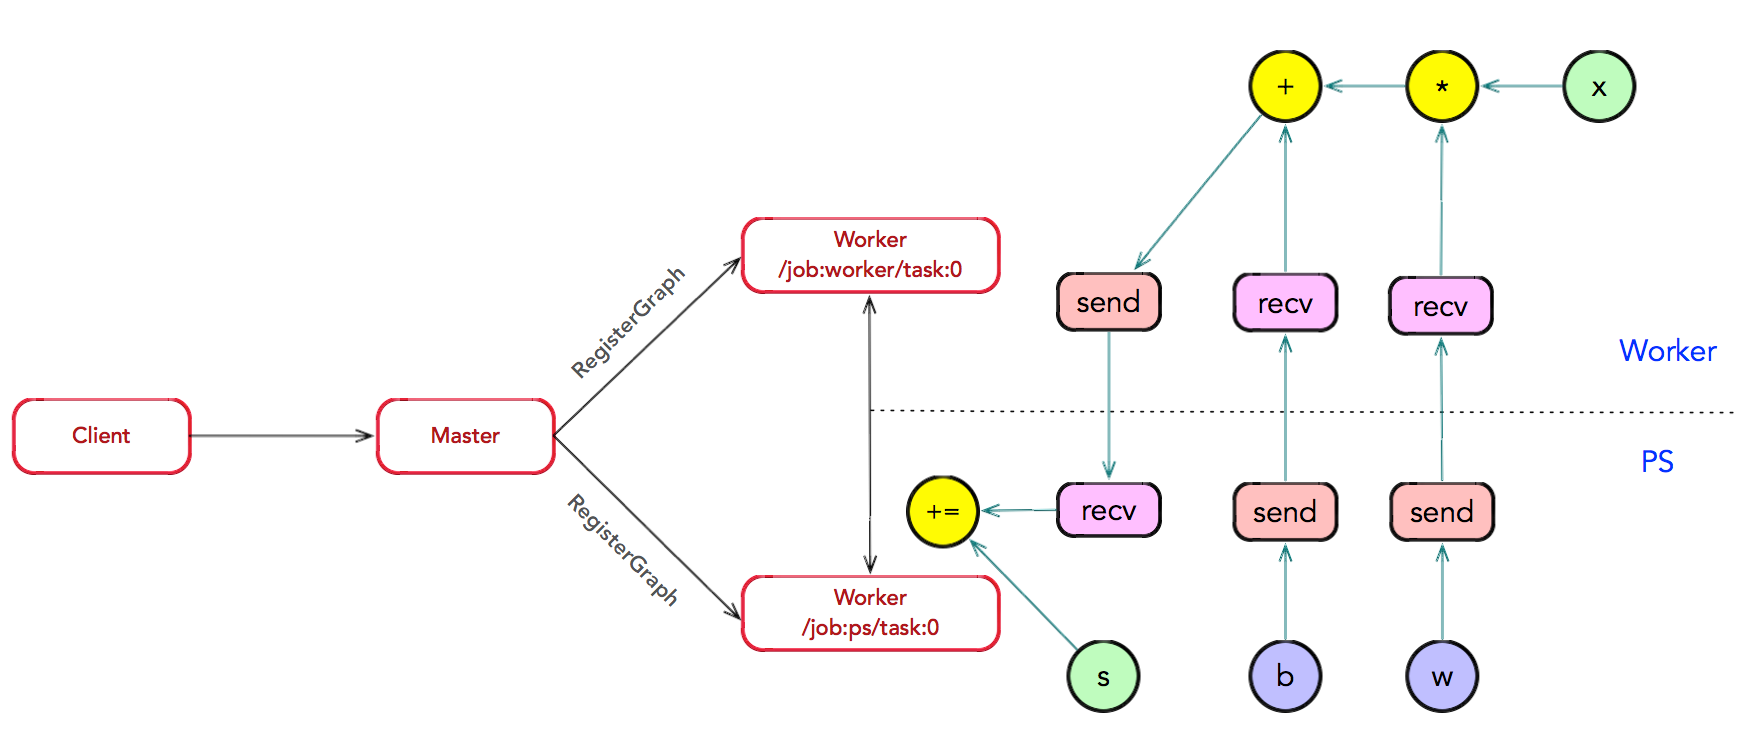
\includegraphics[width=0.9\textwidth]{figures/tf-register-graph.png}
\caption{子图注册:插入Send和Recv节点}}
 \label{fig:tf-register-graph}
\end{figure}

\subsubsection{子图运算}

如\refig{tf-run-graph}所示。\ascii{Master}通过调用\code{RunGraph}接口,通知所有\ascii{Worker}执行子图运算。其中,\ascii{Worker}之间通过调用\code{RecvTensor}接口,完成数据的交互。

\begin{figure}[!htbp]
\centering
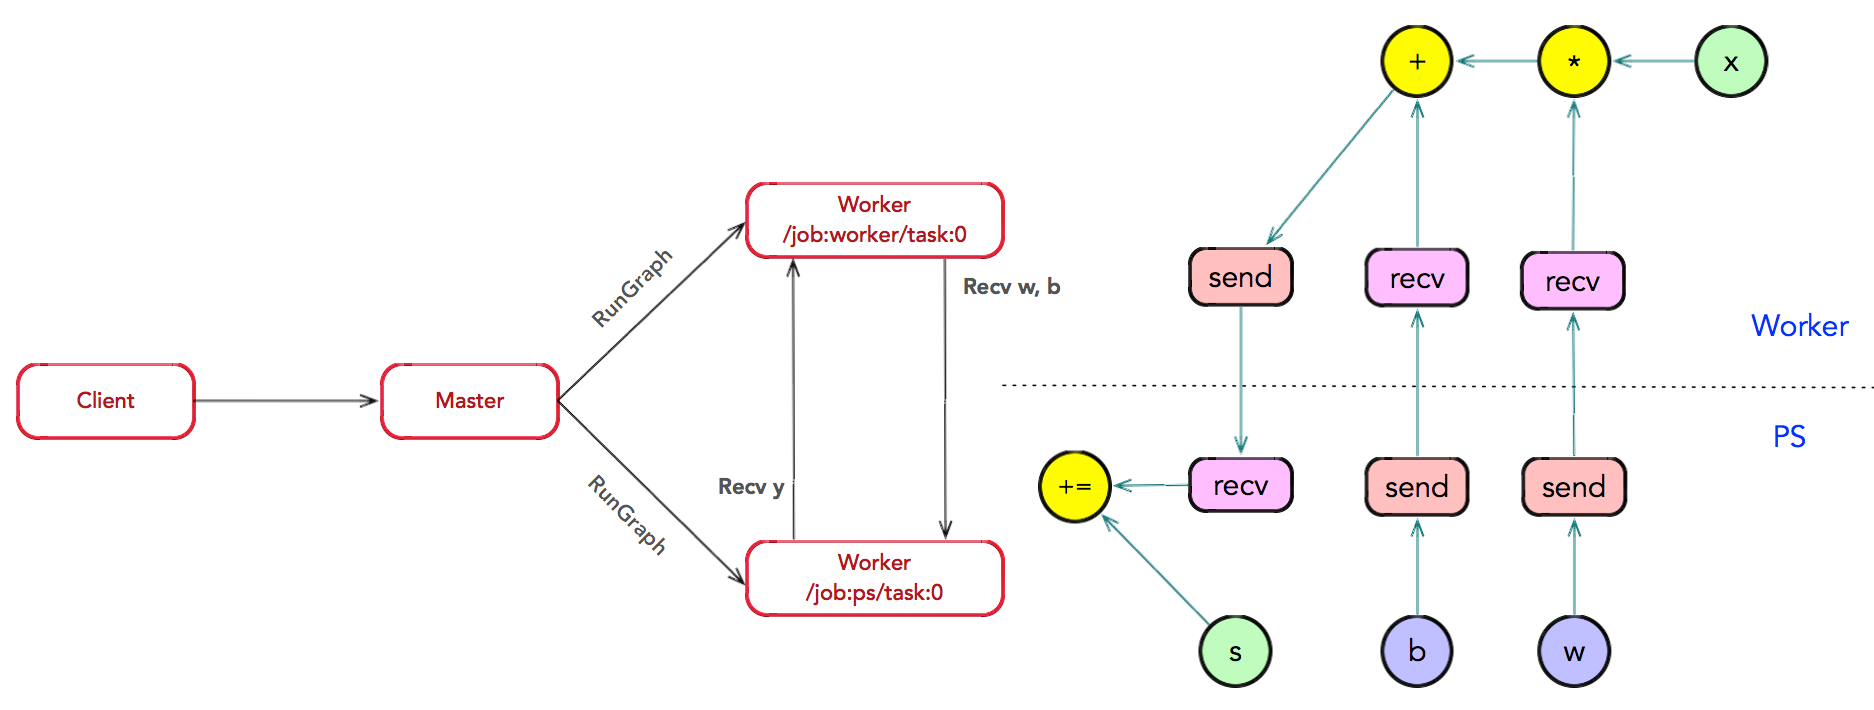
\includegraphics[width=0.9\textwidth]{figures/tf-run-graph.png}
\caption{子图执行}}
 \label{fig:tf-run-graph}
\end{figure}

\end{content}












